\begin{frame}
	\frametitle{Design: high level idea}
	\begin{itemize}
		\item Seed store is a FIFO queue in most AFL based fuzzers, seed explosion could greatly impact fuzzing performance.
		\item A seed has two objectives:
		      \begin{itemize}
			      \item Explore the code, ``exercising an entirely different function'', need less sensitive feedback.
			      \item Exploit the code, focus on solving a particular branch predicate, need more sensitive feedback.
		      \end{itemize}
		\item This is similar to Multi-armed bandit (MAB) problem\footfullcite{10.1145/2508859.2516736}.
	\end{itemize}
\end{frame}

\begin{frame}
	\frametitle{Design: multi level coverage metrics(Sec III)}
	\begin{itemize}
		\item $M_F$: Seeds with the same function coverage
		\item $M_E$: Seeds with the same edge coverage
		\item $M_D$: Seeds with the same hamming distance
	\end{itemize}

	\begin{figure}
		\centering
		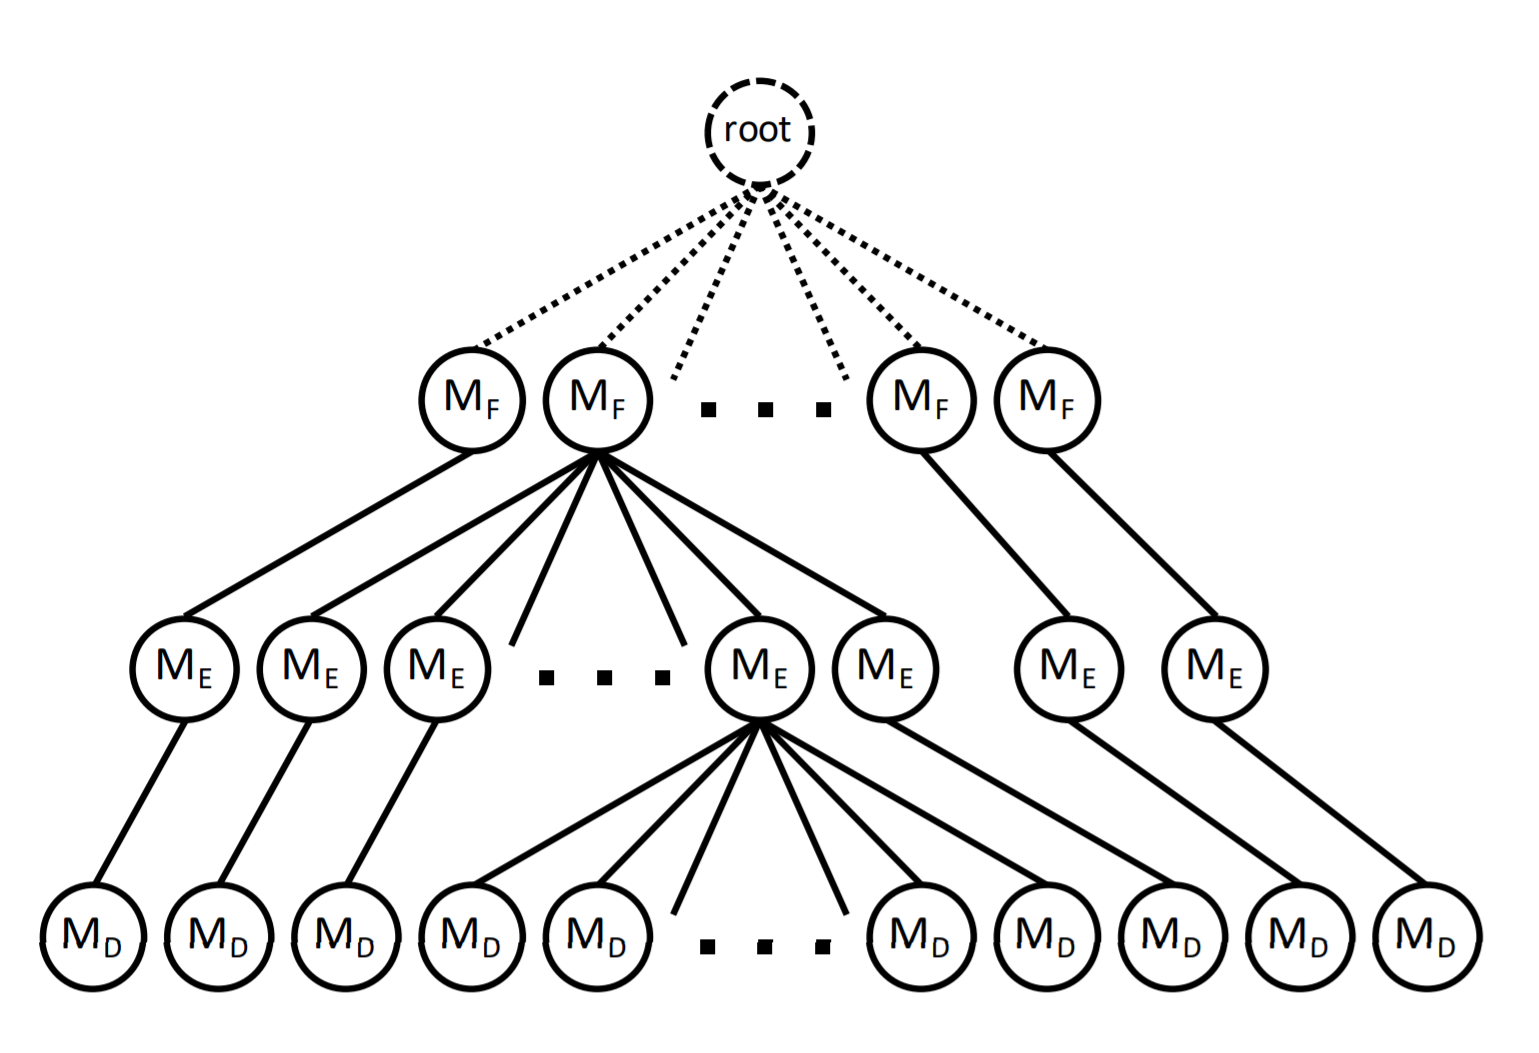
\includegraphics[width=0.5\textwidth]{figs/seedtree.png}
	\end{figure}

	Without FIFO queue, how do we know which seed to take next?
\end{frame}

\begin{frame}
	\frametitle{Design: Hierarchical seed scheduling}
	\begin{itemize}
		\item Seed are scheduled based on their score (Algorithm 3)
		\item $\texttt{Score}(a) = \texttt{Rareness}(a) \times (\texttt{Reward}(a) + \texttt{Uncertainty}(a))$
		\item $\texttt{Rareness}(a)$: Measures how rare is the seed? (Equation 6, 7)
		\item $\texttt{Reward}(a)$: How much reward has the seed gained? (Equation 4)
		\item $\texttt{Uncertainty}(a)$: Radius of the upper confidence interval of \texttt{Reward} (Equation 5)
	\end{itemize}
\end{frame}